\documentclass[12pt]{article}
\usepackage{wrapfig}
\usepackage{adjustbox}
\usepackage{array}

\newcolumntype{R}[2]{%
    >{\adjustbox{angle=#1,lap=\width-(#2)}\bgroup}%
    l%
    <{\egroup}%
}
\newcommand*\rot[2]{\multicolumn{1}{R{#1}{#2}}}

\usepackage{hyperref}
\usepackage{amsmath}
\usepackage{amssymb}
\usepackage{amsfonts}
\usepackage{dsfont}
\usepackage{url}
\usepackage[a4paper,left=1in,top=1in,right=1in,bottom=1in,nohead]{geometry}
\usepackage[round]{natbib}
\usepackage{multirow}
\usepackage{algpseudocode}
\usepackage{algorithm}
\usepackage{subcaption}


\newcommand{\query}{q}
\newcommand{\strsent}{s}
\newcommand{\strsents}{\mathcal{S}}
\newcommand{\nugget}{n}
\newcommand{\extract}{a}
\newcommand{\salience}{y}
\newcommand{\Salience}{Y}
\newcommand{\similarity}{k}
\newcommand{\Similarity}{K}
\newcommand{\updates}{\mathcal{U}}
\newcommand{\nuggets}{\mathcal{N}}
\newcommand{\exemplars}{\mathcal{E}}



\newcommand{\tfidf}{tf-idf }





\newcommand{\poi}{T}

\title{\textbf{What to Write and How to Write It}\\
       \textit{\large Modeling Content Selection and Generation for Text Summarization}\\
       ~\\
       ~\\\large\textbf{Thesis Proposal}}
\author{~\\
        \textbf{Chris Kedzie}\\
        Department of Computer Science\\
        Columbia University\\
        \url{kedzie@cs.columbia.edu}}

\date{December $10^{\textrm{th}}$, 2018}

\begin{document}

\pagenumbering{gobble}
\maketitle

\pagebreak

\renewcommand{\thepage}{\roman{page}}
\setcounter{page}{1}

\begin{abstract}
Automatic text summarization is a long standing NLP problem that has recently 
seen an uptick in interest due to flexible, high capacity deep learning based 
sequence-to-sequence transduction models. 
While many researchers are turning to complex neural networks to perform
end-to-end summary generation, we argue that this unnecessarily obscures
the underlying sub-tasks for summarization. Instead, we propose an alternative
research agenda, focusing on two key summarization subtasks: 
\textit{i)} estimating the general importance of text content for summary 
inclusion, and \textit{ii)} generating text that is faithful, a notion we 
formally define, to said important content. With respect to problem \textit{i)}
we propose several novel methods for working in both low context, streaming
news scenarios, as well as, standard single document summarization settings,
including feature-based and deep learning models of content importance.
On the latter problem, we study the utility of using extractive 
summarization algorithms as a preprocessing stage for a sequence-to-sequence 
based abstractive summarizer, and finally introduce a novel algorithm for
generating text that is faithful, i.e. respects prior beliefs about structured 
knowledge in a database, in an effort to provide stronger guarantees 
about summary reliability.
\end{abstract}

\pagebreak

\tableofcontents
\newpage

\renewcommand{\thepage}{\arabic{page}}
\setcounter{page}{1}
\section{Introduction}

Everyday we ask friends and colleagues to do it, to tell us about books, 
newspaper articles, and other complex pieces of text, and, without more than a 
moment's reflection, they are able to compress their experience
into succint statements in natural language that adequately sum up the thing
being described. The ease with which we summarize belies the difficulty in 
writing programs that do so automatically, and so it would appear that 
the robust
ability to create summaries is, as of 2018, a uniquely human capability.
This partially explains its allure to the artificial intelligence (AI)
research community, which has in one way or another, attempted to aggregate
and naturally compress text data since at least the 1950's 
\citep{luhn1958automatic}.
This makes automatic text summarization one of the longest-standing 
application areas in the 
field of natural language processing (NLP), with a history as long and varied
as some of the more foundational tasks, e.g. parsing and tagging. 

While there are many variants, 
the general summarization task is 
to reduce a large input text into its most essential pieces of information,
and in doing so reduce the amount of reading a human has to do. 
In this thesis we focus on advances to two summarization subtasks:
\textit{(i)} identifying the most import content for inclusion in the summary, 
and \textit{(ii)}
rendering that content in such a way as to not misrepresent the original 
input. We refer to the former as \emph{salience estimation} and the latter
as \emph{faithful generation}. 

The completed and proposed methods of salience estimation cover a range of
techniques including feature-based regression, clustering, learning-to-search,
and deep learning. We experimentally verify the utility of our approaches
across a variety of summarization tasks including stream summarization,
single-document summarization, and multi-document summarization.
The general research goal here is to develop flexible models for 
identifying
important words, phrases, and sentences that are likely to serve as 
representitive members of the larger text in which they are found.

In \emph{extractive summarization}, 
where the summary is constructed by copying and pasting phrases or sentences 
from the input text, salience estimation can be used directly to create
a summary. For example, a simple method of sentence extractive summarization
would be to order the input sentences in decreasing salience and select the
top few sentences for the summary. In most cases, salience is not the only
consideration for summary inclusion; redundancy, discourse coherence, fluency,
and many other metrics of text quality can and have been used as content
selection criteria. These measures are largely independent of salience 
(with the noteable exception of redundancy) and so we do not explore them in 
detail here). Our salience estimation methods will constitute the bulk of the
proposed thesis, the details of completed and proposed work can be found
in \autoref{sec:chapter3} and \autoref{sec:chapter4}.

In \autoref{sec:chapter3} we develop two feature-based models of sentence
salience and evaluate them in a relatively novel \emph{stream summarization} 
crisis-monitoring scenario
\citep{starbird2013working,aslam2016trec}. In this task, a user is interested
in tracking information about a disaster event (e.g. a hurricane). The
user provides a text based query describing the event 
(e.g. ``Hurricane Sandy'') and the summarization model must then 
monitor a stream of news articles, identifying important sentences in the 
document stream and presenting them to the user. The information must be 
highly salient to the query event, as well as novel to the user, and timely
-- we do not want to bombard the user with irrelevant or repeated information,
and our methods used cannot take so long to identify content that the 
information found is out of date.
  
We develop and compare several deep learning based models of word and 
sentence salience in \autoref{sec:chapter4} and evaluate them primarily on
sentence extractive \emph{single document summarization} (SDS). 
We perform this evaluation across
a variety of genres including news, personal narratives, and medical journal
articles. Intuitively, the goal here is to summarize a single news article, 
short story, or research paper by selecting a subset of the input sentences
to serve as the summary. We also explore adaptation of these algorithms to 
the sentence extractive \emph{multi-document summarization} (MDS) task, 
where there is much less data, and only in the news genre.
This is similarly straightforward, given a set of related news articles 
(typically ten), select a subset of the sentences to use as the summary of
the document set.


Salience estimation can also be used to guide 
\emph{abstractive summarization} techniques, i.e. methods that produce novel
summary text using a generative model. These types of models 
must (at the very least) implicitly select important content for conditioning 
their
generative process, and salience estimation can be used for precisely this 
purpose. 

Research in abstractive summarization is increasing, in part due to
the success of general purpose sequence-to-sequence transduction models 
in machine translation (MT) that have been ported to the summarization task.
The ability of abstractive models to generate relatively fluent and 
meaningful summaries is impressive. However, they are also especially prone 
to generating generic statements that are not grounded by evidence in the 
input. This seems to be a well known problem among researchers working
in generation, but it has not received much attention in the literature.
We are interested in this problem from both the perspectives of selecting
the right evidence in the input for generation, a task for which we enlist
our salience estimation methods, and also certifying that a generated text
conforms to knowledge represented in the input or possesed by the model
apriori. For the latter goal, we propose to model generation as a two player
game, where one player, the generator, is tasked with producing a text
utterance describing a piece of evidence (either text or structured data);
the second player, the recognizer, %change this name
evaluates the plausibility of the utterance with respect to the evidence.
This overall regime will consitute our method of faithful generation,
to be outlined in more detail in \autoref{sec:chapter5}. We propose 
evaluation both on an SDS task, as well as, a data-to-text generation 
test bed \citep{wiseman2017challenges}.

\subsection{Contributions}

To summarize, our comleted and proposed contributions of this thesis are as 
follows:
\begin{enumerate}

 \item Two novel feature-based models of sentence salience and an empirical
    evaluation in a stream summarization task.
% \item A novel approach to streaming summarization using a feature-based
%     regression model of sentence salience and sentence selection using 
%     exemplar-based clustering.

% \item A novel approach to streaming summarization using the locally optimal
%     learning to search (LOLS) algorithm.

 \item Several novel deep learning architectures for word and sentence 
   salience, as well as a thorough evaluation of the linguistic and
   structural features critical to learning in the SDS task across a 
   variety of genres.

 \item Adaptation of the deep learning based SDS models to a news MDS task. 

 \item A novel training regime for generative models of text to ensure
          faithfulness of text output to structured data or 
         prior distributions over structured data.

 \item A novel method of combining salience estimation based extractive 
     summarization with abstractive generation in the faithful generation
    paradigm.    

%An experimental evaluation of several existing and novel deep learning
%   architectures for word and sentence salience with 
%A study on the design, strengths, and limitations of deep learning 
%     models for content selection at the sentence and word level in 
%     single document summarization. 

% \item An experimental study of extractive content selection algorithms
%     as input to abstractive summarization model.

% \item A novel approach to generating text that is faithful to some
%     structured information in a database.

\end{enumerate}




%The first two contributions focus broadly on estimating content importance
%or salience for various summarization tasks and domains. They further
%can be broken down into traditional feature-based models (the first two 
%contributions) and deep learning models (the third contribution).
%The last two contributions focus on generating text from previously 
%selected content, with the fourth contribution studying the case where
%selected content consists of extracted sentences and words from an input
%document, and the final contribution focuses on generating text that is 
%faithful to some structured information. 

Together, these contributions
provide a recipe book for identifying summary worthy information and 
generating text that respects truth statements about that information.
The hope is that these methods will lead to more reliable summaries
without sacrificing the expressiveness of the generation algorithm. 

In the next section we describe related work (Section 2). Section 3 describes
completed work on the feature-based approaches to sentence salience estimation.
In section 4, we describe completed and ongoing work on deep learning models
of salience estimation. We describe our planned approaches to faithful 
generation in section 5. Section 6 describes our research plan, before 
we finally conclude.





\section{Related Work}


The complete range of methods and task variations covered by the summarization
literature are too numerous to describe completely here. In the space 
available, we give an overview of unsupervised and supervised learning
approaches to estimating word and sentence importance. 
We also give some background on the variety
of summarization tasks, and the manner in which they are evaluated.


\subsection{Unsupervised Word Importance}


The most obvious signal available for estimating word importance is word 
frequency, i.e. frequent word occurences (modulo stopwords) are likely 
to be related the important topics of the document or document collection 
\cite{topic_sigs}, and it is the chief ingredient in all of the following
word importance estimators.
Term weighting schemes from information retrieval
have frequently been used, most commonly tf-idf 
\cite{centroid,maybe_conroy,find_others}. 
Various probabilistic weightings have also been considered, e.g. the
observed document probability \cite{freq_sum} or the ratio of background
corpus probabiltiy to document probability \cite{topic_sigs}.
Information theoretic transformations of word frequency like the document
level term entropy
have also been found to be useful \cite{klsum,reference_less_summarization}.
Latent semantic analyis (LSA), latent dirichlet allocation (LDA), and
other matrix factorization schemes have been used to find a low dimensional
``concept'' representation for each word, the sum of the concept contributions
constituting the word importance score \cite{multiling_stuff}.
Finally, various methods of transforming word co-occurences into a word graph
have been used in conjunction with unsupervised graph ranking algorithms
\cite{lexrank,conroy_multiling,zhao_2009}.


\subsection{Unsupervised Sentence Importance}

 Graph based ranking that has been used for word importance has similarly 
been used to estimate sentence importance, where the graph consists of 
sentence vertices and edge weights are computed using pairwise sentence 
similarity \cite{textrank}. Another popular method is the centroid method
\cite{centroid} where an average vector representation for a document set is 
constructed and sentences are ranked by their similarity to the centroid object.
Sentence clustering methods have also been applied. In all these methods, 
sentences are tpyically represented as term vectors where the weights for 
each term item are determined by one of the methods mentioned in word importance
estimation methods. 


\subsection{Supervised Word Importance}

The growing availibilty of large text collections with summaries has also
encouraged the development of many supervised methods for learning the word 
importance 
directly from the data. \cite{Regsum} use many of the unsuperivsed word  
importance measures, (e.g. frequency, entropy, document position) to estimate
the probabiltiy of a word occuring in a human abstract. Learning-to-rank
has also been explored in a variety of contexts. For example in single
document summarization, \cite{lapata} used convolutional neural networks
learn rankings and while \cite{guo,macreadie} use a feature based model
to rank sentences in a streaming summarization task.
Word importance weights have also been learned in combinatorial optimization
based approaches to summarization; in several integer linear program (ILP)
formulations of the summarization problem unigram and bigram weights 
are learned \cite{gillick,martens,berkely}, in addition to learning based
submodular optimization approaches \cite{submod,svm}.




\subsection{Supervised Sentence Methods}


Structured prediction methods have also been explored. The most common is
to model the sentence selection problem as an integer linear program (ILP)
and learning typically happens in a large margin/structured svm framework 
\cite{durret}. In addition to learning ngram feature weights, discourse,
and redundancy features can also be modeled \cite{somebody}. 
Deletion based compression 
and phrase substitution have also been modeled using ILPs, where non-essential
phrases can be discarded or shortened, and entity references rewritten, e.g.
turning a pronominal reference into a nominal one.

Sentence selection can be viewed as a submodular set optimization 
(submodularity in set theory is analagous to convexity in functional analysis)
where greedy selection algorithms can efficiently find the best subset of 
sentences according to a set scoring function and budget constraints.
Learning of the scoring function has been done by \cite{uwsipos} using 
linear functions on ngram features. Feature weights can similarly be learned 
in a large margin svm framework.


Sentence selection can be modeled as a sequence tagging problem, e.g. using
hidden Markov models \cite{conroy}.

Dependencies between sentence selection can be difficult, and so in the
spirit of naive Bayes, it can be fruitful to model sentence selection as 
independent classification problems. For example, \cite{kupiec} use ....


\cite{drago_nn} use a graph convolutional neural network on top of a sentence
graph constructed from either discourse structure or sentence similarity.


Learning to rank methods have been explored, see \cite{lapata}.

\subsection{Text Generation}


While there are a variety of text generation methods, we cover three main
approaches, template based generation, sentence fusion, and 
sequence-to-sequence models.



\paragraph{Template-Based Generation} 


\paragraph{Sentence Fusion} Sentence fusion attempts to combine two or
more sentences into one. This is typically done by selecting one sentence
as the backbone, and then aligning the remaing sentences to the backbone.
Heuristics are used for backbone selection and alignment. This method
is better suited to cases where there is much redundancy between candidate
summary sentences since fusing radically different sentences is likely to
yield misleading results.
this approach is that it is difficult 



Thanks to recent advances in neural machine translation (NMT), we now
have flexible, high capacity models for generating free form text from
an arbitrary sequence input. This has led to a host of work exploring 
variety for attention based models to the summarization task \cite{everybody}.
Adaptations to attention like copying have been found to be helpful for 
handling out of vocabulary terms and controlling for repetitive outputs 
\cite{seeandothers}.
One difficulty with this approach is that is hard to control the output,
spurring additional research in more controllable neural text generation.
Length \cite{lc1,lc2}, sentiment \cite{contr}, and domain \cite{socher_I_think}
have been explored, typically by treating the feature under control 
as a learned embedding that is fed as an additional input into the generator.
\cite{lapata} explore a method similar too our faithful text generation model,
however we intend to explore some differences.




 
\subsection{Other stuff from other sections}
Estimating the salience of words and phrases is core to the problem of 
summarization. For example, \cite{luhn1958automatic} 
noted how the most topically central words in a document occur not too much 
but not
too little, and that,
``the presence in the region of highest frequency of many of the words
 previously described as too common to have the  type  of
 significance being sought would constitute
`noise' in the system.''
Typically, this has been done with heuristically derived word weights
\citep{luhn1958automatic,sparck1972statistical} or feature-based, linear 
models of sentence salience \citep{martins2009summarization,woodsend2010automatic,berg2011jointly,durrett2016learning}.

However, the recent availability of large scale single-document summarization 
data \citep{sandhaus2008new,hermann2015teaching,grusky2018newsroom}. 
With these corpora, and other developments in word embedding representation 
\citep{mikolov2013distributed,pennington2014glove},
many researchers have been developing end-to-end models of both 
abstractive \citep{rush2015neural,chopra2016abstractive,cheng2016neural,nallapati2016abstractive,see2017get,paulus2017deep} and extractive \citep{cheng2016neural,nallapati2016classify,nallapati2016summarunner,narayan2018ranking} summarization.
While the spirit of ``let a thousand architectures bloom'' has spurred much
creativity and performance gains, it has left us with little explainability
about how such models work. 

While different components of the neural architectures may be justified 
by intuition, these methods are largely black boxes and it is not clear
how they are making their sentence selection predictions. This is especially
problematic in abstractive summarization, but it is also not well understood
how extractive methods make their decisions either.




~\\
~\\





Subsequently, many methods have been proposed for salience estimation
in the context of summarization. Word weights have typically been derived
in an unsupervised way from a large collection of in-domain text.
The classic example here is Term Frequency-Inverse Document Frequency
(\tfidf) weighting \citep{sparck1972statistical}, whose aim is similar in 
spirit to Luhn's: important 
words occur frequently in the current context (the term frequency component)
 but not so much that they occur in every document 
(the inverse frequency component).

While \tfidf weights (and others like BM25 \citep{bm25}) have been frequent
ingredients in many summarization systems \citep{a,b,c,d,e}, they are 
not specifically tuned to any one summarization task. Another prominent
strand of research has been the learning of word or ngram specific weights
typically for use in linear models of salience \citep{martins2009summarization,woodsend2010automatic,berg2011jointly,durrett2016learning}. 
Given the small size of most summarization datasets at the time, one could question 
the utility of learning ngram weights when it was unlikely that there 
would be adequate data to learn broad coverage summarizers.

%In this chapter we investigate neural network architectures for extractive
%summarization, in the hopes of better understanding what is important 
%for the underlying word and sentence representations to learn.
%We start a description of completed experiments for sentence extractive
%models of summarization \citep{kedzie2018deep}, and then complete the chapter with a description
%of planned and ongoing word importance estimation techniques using deep
%learning models.


~~\\
~\\






Increasingly, researchers are returning to single document summarization,
once thought to be too difficult for automatic summarization methods.
This has been driven both by the availability of large corpora (the
most popular corpus, CNN-DailyMail, has a little over 300,000 data points
\citep{see2017get}) and by the development of general purpose 
generative models of text from the neural machine translation community.
Accordingly, the bulk of the research has used this corpus, (and the NYT
corpus \citep{sandhaus2008new}) to focus on abstractive summarization
research \citep{rush2015neural,chopra2016abstractive,cheng2016neural,nallapati2016abstractive,see2017get,paulus2017deep}. 
There has been a smaller but similar proliferation of sentence
extractive single document summarization papers on these corpora also using 
neural network architectures \citep{cheng2016neural,nallapati2016classify,nallapati2016abstractive,narayan2018ranking}.



\section{Content Selection Models for Streaming Summarization}
This section describes completed work on streaming summarization. We
present two approaches, one using affinity propagation (AP) clustering and 
regression \cite{some_clustering,and_regression},
and one using learning-to-search (L2S) \cite{lols}. 
This work let to two publications \cite{us1,us2} and participation in the
Temporal Sumarization track at the Text REtrieval Conference (TREC)
in 20?? and 20??. The first year, our AP clustering was the best
overall performer, and in the second year, our L2S approach was the 
??? best overall system.





In the streaming summarization task, a user supplies a query $\query$,
a brief text-based search query describing an information need, 
and time period of interest $\poi = (\tau_\alpha, \tau_\omega)$. 
The goal of the task is to sequentially process a document stream 
$X_1, X_2, \ldots$ consisting of an ordered series of
documents with corresponding timestamps $\tau_1, \tau_2, \ldots$,
extracting sentences from the document stream. We refer to the selected
sentences as updates. The document stream is ordered by timestamp where
$\tau_\alpha \le \tau_i \le \tau_\omega$ for all $i$ and $\tau_i \le \tau_j$
for all $i < j$, .


In the Temporal Summarization track, the grounding scenario was disaster
summarization, where the queries corresponeded to natural and man-made 
disasters, and the document stream consisted of online news.
Each query was associated with a set of \textit{nuggets}, textual 
descriptions of canonical pieces of important information for the query event.
See Figure~\ref{fig:events_nuggets} for an example of some of the queries and 
their nuggets. The nuggets are also assumed to have a canonical timestamp
when they are believed to have first been described by a document in 
the document stream.




\begin{figure}
    \textbf{Hurricane Shandy}\\
    ~~~~~~~~~``1986 people left without desert'' ~~ $\cdot$ ~~ ``crane brothers knocked over'' ~~ $\cdot$ ~~ ``subway is better than it will be in 2018''
    Something else \\
    something elses nuggets
    \caption{Example queries in bold, and their nuggets in quotes.}
    \label{fig:events_nuggets}
\end{figure}

Systems are rewarded when they find sentences that contain important and novel
pieces of information relevant to $\query$. Systems are penalized for 
selecting sentences that are irrelevant or contain content already covered
by previous updates. Latency penalized metrics are also computed where
the importance of a nugget decays over time. E.g. if a system
recovers the nugget ``25 people were reported injured,'' several days
after this fact was first reported, it receive less credit for it
than the system that emits that nugget an hour after it enters the 
document stream.


When considering whether or not to select a sentence for the update summary
there are two considerations. First we must estimate the salience, or 
importance, of the sentence with respect to the query. Second, we must consider
whether the relative importance of the sentence in the context of previous
updates and current candidate updates warrants selecting it for the summary.

Streaming summarization is a very hard task compared to single and 
multi-document summarization. In the latter case, the context for the 
summarization is fixed, and the input documents are usually quite 
topically focused, minimizing the prevalence of completely irrelevant 
information. In fact, in most multi-document evaluation settings, the
document collections were manually created leading to very topically
coherent text collections. 
\cite{that_guy_who_presented_once} for example found that in the ???
query focused summarization datasets are so on topic that a summarization
system could completely ignore the query and perform just as well as a
query aware system.





In the next sections, we describe to proposed solutions to this problem.
Both approaches use feature-based regression models to eestimate sentence
salience and so we briefly describe the features here.

\subsection{Features for Sentence Importance Estimation}

The streaming summarization problem is difficult precisely because the context
is constantly shifting. We cannot rely solely on word frequency because
the counts of particular ngrams will be shifting throughout the period of 
interest. Instead we compute several groups of sentence features that are
specifically helpful for the query focused task.

\paragraph{Simple Surface Features} 

We employ several basic features
that have been used previously in supervised
models to rank sentence salience (Kupiec et al.,
1995; Conroy et al., 2001). These include sentence
length, the number of capitalized words normalized
by sentence length, document position,
and number of named entities. The data stream
comprises text extracted from raw html documents;
these features help to downweight sentences
that are not content (e.g. web page titles,
links to other content) or more heavily weight important
sentences (e.g., that appear in prominent
positions such as paragraph initial or article initial).


Our most basic features look at the length in
words of a sentence, its position in the document, and the ratio
of specific named entity tags to non-named entity tokens.
We also compute the average number of sentence tokens that
match the event query words and synonyms using WordNet.


\paragraph{Query Features} Query features measure the
relationship between the sentence and the event
query and type. These include the number of
query words present in the sentence in addition to
the number of event type synonyms, hypernyms,
and hyponyms using WordNet (Miller, 1995). For
example, for event type earthquake, we match sentence
terms “quake”, “temblor”, “seism”, and “aftershock”.


\paragraph{Language Model Scores}



Similar to [Kedzie et al.,
2015], we compute the average token log probability of the
sentence on two language models: i) an event type specific
language model and ii) a general newswire language model.
The first language model is built from Wikipedia articles relevant
to the event-type domain. The second model is built
from the New York Times and Associate Press sections of the
Gigaword-5 corpus [Graff and Cieri, 2003].



Language models
allow us to measure the likelihood of producing
a sentence from a particular source. We consider
two types of language model features. The first
model is estimated from a corpus of generic news
articles (we used the 1995-2010 Associated Press
section of the Gigaword corpus (Graff and Cieri,
2003)). This model is intended to assess the general
writing quality (grammaticality, word usage)
of an input sentence and helps our model to select
sentences written in the newswire style.
The second model is estimated from text specific
to our event types. For each event type
we create a corpus of related documents using
pages and subcategories listed under a related
Wikipedia category. For example, the language
model for event type ‘earthquake’ is estimated
from Wikipedia pages under the category Category:Earthquakes.
Fig. 2 lists the event types
found in our dataset. These models are intended
to detect sentences similar to those appearing in
summaries of other events in the same category
(e.g. most earthquake summaries are likely to include
higher probability for ngrams including the
token ‘magnitude’). While we focus our system on
the language of news and disaster, we emphasize
that the use of language modeling can be an effective
feature for multi-document summarization for
other domains that have related text corpora.
We use the SRILM toolkit (Stolcke and others,
2002) to implement a 5-gram Kneser-Ney model
for both the background language model and the
event specific language models. For each sentence
we use the average token log probability under
each model as a feature.



\paragraph{Geographic Relevance} The disasters
in our corpus are all phenomena that affect some
part of the world. Where possible, we would like
to capture a sentence’s proximity to the event, i.e.
when a sentence references a location, it should be
close to the area of the disaster.
There are two challenges to using geographic
features. First, we do not know where the event is,
and second, most sentences do not contain references
to a location. We address the first issue by
extracting all locations from documents relevant to
the event at the current hour and looking up their
latitude and longitude using a publicly available
geo-location service. Since the documents that are
at least somewhat relevant to the event, we assume
in aggregate the locations should give us a rough
area of interest. The locations are clustered and
we treat the resulting cluster centers as the event
locations for the current time.
The second issue arises from the fact that the
majority of sentences in our data do not contain
explicit references to locations, i.e. a sequence of
tokens tagged as location named entities. Our intuition
is that geographic relevance is important in
the disaster domain, and we would like to take ad


\paragraph{Temporal Relevance} As we track
events over time, it is likely that the coverage of
the event may die down, only to spike back up
when there is a breaking development. Identifying
terms that are “bursty,” i.e. suddenly peaking
in usage, can help to locate novel sentences that
are part of the most recent reportage and have yet
to fall into the background.
We compute the IDF for each hour in our data
stream. For each sentence, the average TF*IDF
for the current hour t is taken as a feature. Additionally,
we use the difference in average TF*IDF
from time t to t − i for i = {1, . . . , 24} to measure
how the TF*IDF scores for the sentence have
changed over the last 24 hours, i.e. we keep the
sentence term frequencies fixed and compute the
difference in IDF. Large changes in IDF value indicate
the sentence contains bursty terms. We also
use the time (in hours) since the event started as a
feature.


\subsection{Model 1: Salience Estimation with Affinity Propagation Clustering}

  In this model, we process the document stream in hourly batches, 
  first predicting the salience of the individual sentences and then 
  using affinity propagation (AP) to select a set of exemplar sentences.
  Exemplar sentences that have predicted salience above a threshold 
  and are below a similarity threshold to previously select sentences are
  then emitted to the user as an update summary.

  
\subsubsection{Data}

  The document stream comes from the news portion of the 2014 TREC
KBA Stream Corpus \cite{frank_et_al_2012}, which contains hourly crawls
of the web covering a roughly two year span from 2011 to 2013.
Event queries and their nuggets were taken from the data prepared for 
the 2013 and 2014 TREC Temporal Summarization tracks. This data
contained 25 events and their query strings, period of interest, 
event type. 
Additionally, each event was associated with anywhere from 50 to several
hundred timestamped nugget texts. Each event query was significant 
enough to have a Wikipedia page. Event nuggets were taken manually
extracted from the corresponding Wikipedia entry, using the earliest
revision that contained the nugget to obtain it's timestamp.
For details on the creation of this dataset see \cite{aslam_et_al_2013}.

From the larger KBA Stream Corpus we created event specific document 
streams by filtering out any documents that did occur in the period
of interest and contain all the query words of the corresponding event.  



\subsubsection{Salience Estimation}

Since we lack annotations 











%During the a tim

%While  An
%information retrieval (IR) system will then begin 















\section{Deep Learning Models of Word and Sentence Salience}

\label{sec:chapter4}

\def\tfidf{TF-IDF}

Estimating the salience of words and phrases is core to the problem of 
summarization. For example, \cite{luhn1958automatic} 
noted how the most topically central words in a document occur not too much 
but not
too little, and that,
``the presence in the region of highest frequency of many of the words
 previously described as too common to have the  type  of
 significance being sought would constitute
`noise' in the system.''

Subsequently, many methods have been proposed for salience estimation
in the context of summarization. Word weights have typically been derived
in an unsupervised way from a large collection of in-domain text.
The classic example here is Term Frequency-Inverse Document Frequency
(\tfidf) weighting \citep{sparck1972statistical}, whose aim is similar in 
spirit to Luhn's: important 
words occur frequently in the current context (the term frequency component)
 but not so much that they occur in every document 
(the inverse frequency component).

While \tfidf weights (and others like BM25 \citep{bm25}) have been frequent
ingredients in many summarization systems \citep{a,b,c,d,e}, they are 
not specifically tuned to any one summarization task. Another prominent
strand of research has been the learning of word or ngram specific weights
typically for use in linear models of salience \citep{martins2009summarization,woodsend2010automatic,berg2011jointly,durrett2016learning}. 
Given the small size of most summarization datasets at the time, one could question 
the utility of learning ngram weights when it was unlikely that there 
would be adequate data to learn broad coverage summarizers.

This 
situation has changed with the recent availability of large scale summarization data \citep{cnndm,newsroom,nyt}. With these corpora,
and other developments in word embedding representation \citep{miklov,glove},
many researchers have been developing end-to-end models of both 
abstractive \citep{abs} and extractive \citep{ext} summarization.
While the spirit of ``let a thousand architectures bloom'' has spurred much
creativity and performance gains, it has left us with little explainability
about how such models work. 

While different components of the neural architectures may be justified 
by intuition, these methods are largely black boxes and it is not clear
how they are making their sentence selection predictions. This is especially
problematic in abstractive summarization, but it is also not well understood
how extractive methods make their decisions either.

In this chapter, we describe completed experiments teasing out the importance
of different neural network designs for sentence level salience. This
work describes impedements to learning and word and sentence representations
in deep learning models of extractive summarization, and led to 
a recent publication \citep{kedzie2018deep}. Based on these limitations,
we propose extensions to the word level representations and explicitly model
word level salience scores as a means to performing sentence extractive
summarization. While the finished and proposed work focuses on single document
summarization, we also propose an extension of the word level salience
estimation model that we hope will generalize to the multi-document
summarization context.


%In this chapter we investigate neural network architectures for extractive
%summarization, in the hopes of better understanding what is important 
%for the underlying word and sentence representations to learn.
%We start a description of completed experiments for sentence extractive
%models of summarization \citep{kedzie2018deep}, and then complete the chapter with a description
%of planned and ongoing word importance estimation techniques using deep
%learning models.


~~\\
~\\






Increasingly, researchers are returning to single document summarization,
once thought to be too difficult for automatic summarization methods.
This has been driven both by the availability of large corpora (the
most popular corpus, CNN-DailyMail, has a little over 300,000 data points
\citep{see2017get}) and by the development of general purpose 
generative models of text from the neural machine translation community.
Accordingly, the bulk of the research has used this corpus, (and the NYT
corpus \citep{sandhaus2008new}) to focus on abstractive summarization
research \citep{rush2015neural,chopra2016abstractive,cheng2016neural,nallapati2016abstractive,see2017get,paulus2017deep}. 
There has been a smaller but similar proliferation of sentence
extractive single document summarization papers on these corpora also using 
neural network architectures \citep{cheng2016neural,nallapati2016classify,nallapati2016abstractive,narayan2018ranking}.



\ifthenelse{\equal{\highlevel}{false}}{
  
\newcommand{\sent}{s}
\newcommand{\Sents}{\mathcal{S}}
\newcommand{\doc}{D}
\newcommand{\lbl}{y}
\newcommand{\Labels}{Y}
\newcommand{\word}{w}
\newcommand{\vocab}{\mathcal{V}}
\newcommand{\extracts}{\mathcal{E}}
\newcommand{\budget}{c}
\newcommand{\encoder}{\textsc{Encoder}}
\newcommand{\extractor}{\textsc{Extractor}}
\newcommand{\embproj}{W}
\newcommand{\emb}{\omega}
\newcommand{\embsize}{n}
\newcommand{\sembsize}{m}
\newcommand{\semb}{h}
\newcommand{\rsemb}{\overrightarrow{\semb}}
\newcommand{\lsemb}{\overleftarrow{\semb}}
\newcommand{\gru}{\textsc{Gru}}
\newcommand{\rgru}{\overrightarrow{\gru}}
\newcommand{\lgru}{\overleftarrow{\gru}}
\newcommand{\cfeat}[2]{f_{#1}^{( #2 )}}
\newcommand{\relu}{\textsc{ReLU}}
\newcommand{\winsize}{k}
\newcommand{\winsizes}{K}
\newcommand{\fmapsize}{F}
\newcommand{\cfidx}{l}
\newcommand{\cact}{a^{(\cfidx,\winsize)}}
\newcommand{\cnnbias}{u^{(\winsize)}}
\newcommand{\cnnweight}{U^{(\winsize)}}
\newcommand{\cnnBiasSpace}{\mathbb{R}^{\fmapsize_\winsize}}
\newcommand{\cnnWeightSpace}{\mathbb{R}^{\winsize \times \fmapsize_\winsize \times \embsize}}


\subsection{Deep Learning Models of Sentence Extraction}

 Given the diversity of neural architectural choices, a best practices
for sentence extracive summarization has yet to emerge. In this section
we ask what architecture design choices matter for single document 
summarization across a variety of domains.

We begin by definining some terminology. A sentence is represented as an
sequence of words $\sent = \{\word_1, \word_2, \ldots, \word_{|\sent|} \}$
where each word is drawn from a fixed vocabulary $\vocab$ and $|\sent|$ is
the length of sentence $\sent$ in words. Similarly, a document $\doc = \{ 
\sent_1, \sent_2, \ldots, \sent_{|\doc|} \}$ is a sequence of sentences, where 
$|\doc|$ is the size of the document in sentences.  

We treat the sentence extractive summarization as sequence tagging
problem: given a document $\doc$, we want to assign an associated binary
tag sequence $\Labels = \{\lbl_1, \lbl_2, \ldots, \lbl_d \}
\in \{0,1\}^d$ such that the extract summary $\extracts = \{ 
\sent_i \in \doc : \lbl_i =1 \}$ implied by $\Labels$ is a suitable summary
of the document. Typically, it is assumed that size of the extract summary
$|\extracts| = \sum_{i=1}^{|\doc|} \mathbbm{1}\{\lbl_i =1 \} \ll |\doc|$.
It is also common to enforce a word budget $\budget$ such that
$\sum_{\sent \in \extracts} |\sent| \le \budget$.

A typical deep learning model will build up a hierarchical representation
of each sentence, starting at the word level, and then composing an arbitrarily
long sequence of word representations into a fixed length sentence 
representation.
First the individual words are 
projected to fixed length vectors, or word embeddings via a mapping
$\embproj : \vocab
\rightarrow \mathbb{R}^{\embsize}$. The sentence encoder network $\encoder :
\{\mathbb{R}^{\embsize}\}^* \rightarrow \mathbb{R}^{\sembsize}$ is then 
responsible for mapping word embbeding sequences to fixed length sentence 
embeddings. Finally, the sentence extractor network $\extractor : 
\{\mathbb{R}^\sembsize\}^* \rightarrow \{0, 1\}^*$ produces a label 
sequence $\Labels$.

We explore several choices of encoder and extractor architecture from the 
literature \citep{cheng2016neural,nallapati2016summarunner} as well as 
propose our own designs \citep{kedzie2018deep}. In the next sections,
we describe the three sentence encoder architectures (\textit{avg}, 
\textit{rnn}, and \textit{cnn}) followed by four extractor architectures 
(\textit{rnn}, \textit{seq2seq}, \textit{sr}, and \textit{cl}).

\subsubsection{Sentence Encoders}
\paragraph{Averaging} The simplest encoder simply averages a sentence's
associated word embeddings:
\[ \encoder_{avg}(\sent) = \frac{1}{|\sent|} \sum_{\word \in \sent} \embproj(\word). \]
Other than the word embeddings, this encoder involves no learned parameters,
and while it collapses word order, embedding averaging has consistently
been found competitive with more sophisticated sentence embedding techniques
\citep{iyyer2015deep,wieting2015towards,arora2016simple,wieting2017revisiting}.


\paragraph{Recurrent Neural Networks} The second encoder architecture
we experiment with is a recurrent neural network (RNN) over the word
embeddings. An RNN maintains an internal ``hidden'' state that is sequentially
updated upon observing each word embedding. In practice, we use a bidirectional
RNN with a gated recurrent unit (GRU) as the particular instantiation of 
the RNN cell \citep{cho2014learning}.
Under the RNN encoder, a sentence embedding for a sentence $\sent$ is defined 
as
\begin{align}
\encoder_{rnn}(\sent) = [\overrightarrow{\semb}_{|\sent|}, \overleftarrow{\semb}_{1} ] & \\
  \rsemb_0 = \mathbf{0};& \quad 
  \rsemb_i = \rgru\left(\embproj(\word_i), \rsemb_{i-1}\right) \\
  \lsemb_{|\sent| + 1} = \mathbf{0};& \quad 
  \lsemb_i = \lgru\left(\embproj(\word_i), \lsemb_{i+1}\right) 
\end{align}
where $[\cdot]$ is the concatenation operator; $\rsemb_i$ and $\lsemb_i$ are
hidden states of the forward and backward GRU cells respectively; and 
$\rgru, \lgru : \mathbb{R}^\embsize \times \mathbb{R}^\sembsize 
\rightarrow \mathbb{R}^\sembsize$ are the forward and backward GRU cell 
operations.
\cite{nallapati2016summarunner} use a bidirectional RNN for their sentence
encoder.

\paragraph{Convolutional Neural Networks}
Our final sentence encoder uses a convolutional neural network
(CNN) to encode important ngram windows into a fixed length vector. 
CNN's have grown increasingly popular in many NLP tasks 
as a computationally efficient substitute for RNN-based architectures
\citep{kim2014convolutional,lei2015molding,dauphin2017language}.
Our architecture largely follows \cite{kim2014convolutional}: we apply a 
series of one dimensional convoluions over a sentence's word embeddings
using varying width convolutions. For each convolutional window size 
$\winsize \in \winsizes \subset \mathbb{N}$, a convolutional filter creates 
a feature vector $\cfeat{}{\winsize} \in \mathbb{R}^{\fmapsize_\winsize}$ 
and the encoder output is the concatenation of the $|\winsizes|$ vectors. 
The set of filter window sizes $\winsizes$ and the number of feature maps
$\fmapsize_\winsize$ for each $\winsize \in \winsizes$ are 
model hyperparameters.
Formally, we define the CNN encoding of a sentence $\sent$ as 
\begin{align}
\encoder_{cnn}(\sent) & = \left[\cfeat{}{\winsize} : \winsize \in \winsizes \right]\\
\cfeat{\cfidx}{\winsize} &= 
     \max_{i \in 1,\dots, |\sent| - \winsize + 1} 
       \relu\left(\cact_i \right) \\
\cact_i &= \cnnbias_\cfidx
    + \sum^{\winsize}_{j=1} \cnnweight_{\cfidx,j} \cdot \embproj(\word_{i + j -1})
\end{align}
where $\cnnbias \in \cnnBiasSpace$ and $\cnnweight \in \cnnWeightSpace$
are learned convolutional filter weights and $\relu(x) = \max(0, x)$ 
is the rectified linear unit \citep{nair2010rectified}. \cite{cheng2016neural}
uses a CNN for their sentence encoder.

\subsubsection{Sentence Extractors}

A sentence extractor takes the encoder output, i.e. 
a sequence of sentence embeddings
$\encoder(\doc) =$ $\{\encoder(\sent_1), \ldots, \encoder(\sent_{|\doc|})\} =
\{\semb_1, \ldots, \semb_{|\doc|}\}$, and produces a sequence of labels
$\Labels = \{\lbl_1, \ldots, \lbl_{|\doc|}\}$. 
The sentence extractor is essentially a discriminative
classifier $p(\lbl_1,\ldots,\lbl_{|\doc|} | \semb_1,\ldots,\semb_{|\doc|})$.
Previous neural network approaches to sentence extraction have assumed
an auto-regressive model, leading to a semi-Markovian
factorization of the extractor probabilities
$p(\lbl_{1:n}|\semb)=\prod_{i=1}^{|\doc|} 
p(\lbl_i|\lbl_{<i},\semb)$,
where each prediction $\lbl_i$ is dependent on \emph{all}
previous $\lbl_j$ for
all $j < i$. We compare two such models proposed by \cite{cheng2016neural}
and \cite{nallapati2017summarunner}.
A simpler approach that does not allow interaction among the $\lbl_{1:n}$
is to
%\hal{a simpler approach (explain why simpler) is a fully factored representation 
  model $p(\lbl_{1:n}|\semb) = \prod_{i=1}^n p(y_i|h)$,
  which we explore in two proposed extractor models that we refer to as the RNN 
  and Seq2Seq extractors.
%Implementation details for all extractors are in \autoref{app:sentextractors}.


%\paragraph{Previously Proposed Sentence Extractors}
% We consider two recent state-of-the-art extractors.
\paragraph{Cheng \& Lapata Extractor} 
 The first extractor we consider, proposed by 
\citet{cheng2016neural}, %, which we refer to as the Cheng \& Lapata Extractor,
is built around a sequence-to-sequence model.
First, each sentence embedding\footnote{\citet{cheng2016neural} used an CNN sentence encoder with 
this extractor architecture; in this work we pair the Cheng \& Lapata extractor
with several different encoders.} is
fed into an encoder side RNN, with the final encoder state passed to the
first step of the decoder RNN. On the decoder side, the same sentence 
embeddings are fed as input to the decoder and decoder outputs are used to
predict each $\lbl_i$. The decoder input is weighted by the previous extraction
probability, inducing the dependence of $\lbl_i$ on $\lbl_{<i}$.
See \autoref{fig:extractors}.c for a graphical layout of the extractor.
%and \autoref{app:clextractor} for details.

%?, but are delayed by one step and 
%?weighted by their prediction probability, i.e. at decoder step $t$,
%?$p(\slabel[t-1]|\slabel[<t-1], \sentEmb[<t-1]) \cdot \sentEmb[t-1]$\hal{why did you switch from $i$ to $t$?}
%?is fed into the decoder\hal{i don't udnerstand what this means. what op is $\cdot$?}. The decoder output at step $t$ is concatenated 
%?to the encoder output step $t$ and fed through a multi-layer perceptron
%?with one hidden layer and sigmoid unit output computing the $t$-th
%?extraction probability $p(\slabel[t]|\slabel[<t], \sentEmb[<t])$. \textcolor{red}{See Figure 2.c. for a graphical view. Full model details are presented in ??}.
%?

\paragraph{SummaRunner Extractor}\citet{nallapati2017summarunner} proposed
a sentence extractor, which we refer to as the SummaRunner Extractor,
that factorizes the extraction probability into contributions 
from different sources.
First, a bidirectional RNN is run over the sentence embeddings\footnote{\citet{nallapati2017summarunner}
    use an RNN sentence encoder with 
this extractor architecture; in this work we pair the SummaRunner extractor
with different encoders. } and the output is
concatenated. A representation of the whole document is made by 
averaging the RNN output. A summary representation is also constructed 
by taking the sum of the previous RNN outputs weighted by their extraction
probabilities. Extraction predictions are made using 
the RNN output at the $i$-th step, the document representation, and 
$i$-th version of the summary representation, along with factors for 
sentence location in the document. The use of the iteratively constructed
summary representation creates a dependence of $\lbl_i$ on all $\lbl_{<i}$.
See \autoref{fig:extractors}.d for a graphical layout.
%

%\paragraph{Proposed Sentence Extractors}
%We propose two sentence extractor models that 
%make a stronger conditional independence 
%assumption $p(\slabel|\sentEmb)=\prod_{i=1}^\docSize p(\slabel[i]|\sentEmb)$,
%essentially making independent predictions conditioned on $\sentEmb$.


\paragraph{$\extractor_{rnn}$}
    Our first proposed model is a very simple bidirectional
RNN based tagging model. As in the RNN sentence encoder we use a GRU cell.
The forward and backward outputs of each sentence are passed through a 
multi-layer perceptron with a logsitic sigmoid output 
to predict the probability
of extracting each sentence. 
See \autoref{fig:extractors}.a for a graphical layout.
%and \autoref{app:rnnextractor} for details.


\newcommand{\rExtHidden}{\overrightarrow{h}}
\newcommand{\lExtHidden}{\overrightarrow{h}}
\newcommand{\docSize}{|\doc|}
\newcommand{\logits}{o}

\begin{align}
    \rExtHidden_0 = \mathbf{0};&\quad   \rExtHidden_i = \rgru(\semb_i, \rExtHidden_{i-1}) \\
    \lExtHidden_{\docSize + 1} = \mathbf{0};&\quad    \lExtHidden_i = \lgru(\semb_i, \lExtHidden_{i+1}) \\
   \logits_i &= \relu\left(U \cdot [\rExtHidden_i; \lExtHidden_i] + u \right)\\
    p(\lbl_i=1|\encoder(\doc)) &= \sigma\left(V\cdot \logits_i + v  \right)
\end{align}
where $\rgru$ and $\lgru$ indicate the 
forward and backward GRUs respectively, and each have separate learned 
parameters; $U, V$ and $u, v$ are learned weight and bias parameters.
The hidden layer size of the GRU is 300 for each direction and the MLP hidden layer
size is 100. Dropout is applied to the GRUs and to $a_i$.





\paragraph{$\extractor_{s2s}$} One shortcoming of the RNN extractor is that long range
information from one end of the document may not easily be able to affect 
extraction probabilities of sentences at the other end. 
Our second proposed model, the $\extractor_{s2s}$ mitigates this problem with an 
attention 
mechanism commonly
used for neural machine translation \cite{bahdanau2014neural} and 
abstractive summarization \cite{see2017get}. 
The sentence embeddings are first
encoded by a bidirectional $\gru$. A separate decoder $\gru$ transforms each 
sentence into a query vector which attends to the encoder output. The
attention weighted encoder output and the decoder $\gru$ output are concatenated
and fed into a multi-layer perceptron to compute the extraction probability.
See \autoref{fig:extractors}.b for a graphical layout.




\subsection{Experiments}

 We are interested in two questions. The first, more pragmatic question, is
 what are the best configuration of encoder/extractor architectures?
 We answer this question by evaluating ROUGE recall and METEOR \citep{meteor}
 performance across our six collected datasets. We perform the standard
 stochastic gradient descent \cite{sgd} based optimization (using the Adam
 update \cite{adam}) of the weighted negative log likehood 
 \[ \mathcal{L}(\theta) = -\sum_{\Sents, \Labels \in \mathcal{D}} 
            \sum_i \omega(\lbl_i) 
        \log p(\lbl_i|\lbl_{<i}, \Sents; \theta) \]
        where $\theta$ are model parameters and $\omega(\lbl_i)$ upweights
        the positive labels to account for the imbalanced label distribution.

 We lack human reference extract labels for our datasets and so we obtain
 said lable sequences heuristically, by finding a label sequence $\Labels^*$
 by greedily optimizing ROUGE-1 recall with respect to the human reference
 abstracts.

 The second question, is more diagnostic in nature: what signals
 in the data are driving model learning?
 We perform several experiments to find answers. 
 We hypothesize that the lexical semantics encoded at the word embedding
 level will be important to subsequent sentence representations, and
 perform a comparison on learning with and with out fine tuning of the 
 embeddings. In both cases, embeddings are initialized with Glove
 embeddings pretrained on Wikipedia and Gigaword \citep{glove}.
 
 
 We also hypothesize that certain classes of words will be more important 
 to identifying salient content than others. We perform word ablation 
 experiments where we alternately remove nouns, verbs, adjectives \& adverbs,
 and function words from the sentence encoder input and compare performance 
 to the non-ablated system. We expect that the nouns will be more important
 to content selection. 


 Our final experiments attempt to tease out the effect of structural features 
 from the lexical. In this experiment, we shuffle the sentence order at 
 training time. In this setup, we obfuscate features about which content 
 was introduced in the article first, an important and well known bias in 
 news domain \cite{leadbias}. 


 \subsection{Results}


  

The results of our main experiment comparing 
the different extractors/encoders are shown in 
Table~\ref{tab:results}.
Overall, we find no major advantage when using the CNN and RNN sentence
encoders over the averaging encoder. The best performing encoder/extractor pair either 
uses the averaging 
encoder (five out of six datasets) or the differences 
are not statistically significant. %When only comparing within the 
%same extractor choice,  the averaging encoder is the better choice
%in 14 of 20 cases. 
%\hal{i wonder if it would be worth adding another ``average performance metric'' column to \autoref{tab:results}.
%  i'm thinking have ``Average $\Delta$-Best'' meaning how far (on average across the datasets) is this setting from the best setting available on that dataset.
%  so since the best numbers are: 25.56, 35.85, 23.11, 13.65, 5.63
%  and the first row numbers are: 25.42, 34.67, 22.65, 11.37, 5.50
%  then the deltas are:            0.14,  1.18,  0.46,  2.28, 0.13
%  the the average delta is 0.84 (assuming my math is right)
%  there's an argument to do multiplicative, in which case
%  the multipliers for first row:  0.99,  0.97,  0.98,  0.83, 0.97
%  and the average is 0.95
%  either way this gives a quick way to make comparisons between rows. you could do the same for the other tables too.}

  %\hal{in some of the tables you list R-2 as headers even though all the numbers are R-2. just put that in the caption.}


When looking at extractors, the Seq2Seq extractor is either part of 
the best performing system (three out of six datasets) or is not 
statistically distinguishable from the best extractor. 

Overall, on the news and medical journal domains, the differences are 
quite small with the 
differences between worst and best systems on the CNN/DM dataset 
spanning only .56 of a ROUGE point. While there is more performance variability
 in the Reddit and AMI data, there is less distinction among systems: 
 no differences are significant on Reddit
and every extractor has at least one configuration that is indistinguishable
from the best system on the AMI corpus. This is probably due to the small test
size of these datasets.
%\hal{this is probably at least partially because of test set size. maybe mention this.}





%?\textcolor{red}{Overall we find that the \modelTwoBF~extractor achieves the 
%?best ROUGE scores on three out of four domains (STILL RUNNING ON AMI AND PUBMED). 
%?However, most
%?differences are not signficant. (Need to discuss stat sig and how to show it).}
%?On the larger CNN-DailyMail dataset, especially, 
%?differences are quite smail across all extractor/encoder pairs.
%?The \baselineOneBF~extractor achieves the best performance on the DUC 2002
%?dataset. It is disappointing that the \baselineOneBF~and \baselineTwoBF~based 
%?models do not gain any apparent advantage in conditioning on previous 
%?sentence selection decisions; this result suggests the need to improve
%?the representation of the summary as it is being constructed iteratively.
%?
%?\textbf{Choice of Encoder} We also find there to be no major advantage 
%?between the different sentence encoders. \textcolor{red}{In most cases,
%?there is no statistical significance between the averaging encoder and either
%?the RNN or CNN encoders.} 

%The lack of differentiation amongst the different encoders concerning; one
%would assume learning with the appropriate structure would be helpful.
%The results of next 




\paragraph{Word Embedding Learning}
 Given that learning a sentence encoder (averaging has no learned parameters)
 does not yield significant improvement, it is natural to consider whether
 learning word embeddings is also necessary. 
 In \autoref{tab:embeddings} we compare the performance of different extractors
 using the averaging encoder, when the word embeddings are held fixed or 
 learned during training. In both cases, word embeddings are initialized with
 GloVe embeddings trained on a combination of Gigaword and Wikipedia.
% \hal{TRAINED ON WHAT? JUST THE DEFAULT ONES?}
 When learning embeddings, words occurring 
 fewer than three times in the training data are mapped to an unknown
 token (with learned embedding).
 
% shows ROUGE recall
%when using fixed or updated word embeddings. 
 In all but one case,
fixed embeddings are as good or better than the learned embeddings.
This is a somewhat surprising finding on the CNN/DM data since it is reasonably
large, and learning embeddings should give the models more
flexibility to identify important word features.\footnote{The AMI corpus is an exception here where learning \emph{does} lead to small
performance boosts, however, only in the Seq2Seq extractor is this diference 
significant; it is quite possible that this is an artifact of the very small
test set size.}
%\hal{why is it surprising?} \textcolor{green}{[[CK: Because learning embeddings should give the model more capacity to represent important patterns]]}
This suggests that we cannot extract much generalizable learning signal 
from the content other than what is already present from initialization. 
Even on PubMed, where the language is quite different from the news/Wikipedia
articles the GloVe embeddings were trained on, learning leads to 
significantly worse results.

%The language of this corpus is quite different from the 
%data that the GloVe embeddings were trained on and so it makes sense 
%that  there would be more benefit to learning word representations; one
%explanation for only seeing modest improvements is purely the small size
%of the test dataset which has only 20 training meetings.

%textcolor{red}{(NOTE TO CK -- expect learning to help on pubmed)}. \hal{yes, the dataset size is certainly an issue here. probably worth pointing this out. also when you learned the embeddings, did you initialize to pretrained embeddings? did you regularize toward them?}


\paragraph{POS Tag Ablation}
It is also not well explored what word features are being used by the encoders.
To understand which classes of words were most important we ran an ablation
study, selectively removing nouns, verbs 
(including participles and auxiliaries), adjectives \& adverbs, and 
function words (adpositions, determiners, conjunctions).
%Additionally, we ran ablation experiments
%using part-of-speech (POS) tags. \hal{this needs to be justified. why is this experiment interesting?}
All datasets were automatically tagged using
the spaCy part-of-speech (POS)
tagger\footnote{https://github.com/explosion/spaCy}.   
%\kathy{I'm still curious what would happen if you separately removed all conjunction tags and later remaining POS.}
%We experimented with selectively removing 
%\begin{itemize}
%    \item nouns (NOUN and PROPN tags), 
%    \item verbs (VERB, PART, and AUX tags), 
%    \item adjectives/adverbs (ADJ and ADV tags), 
%    \item numerical expressions (NUM and SYM tags), and 
%    \item miscellaneous words (ADP, CONJ, CCONJ, DET, INTJ, and SCONJ tags)
%\end{itemize}
%from each sentece. 
The embeddings of removed words were replaced with a zero vector,
preserving the order and position of the non-ablated words in the sentence.
Ablations were performed on training, validation, and test partitions,
using the RNN extractor with averaging encoder.
\autoref{tab:ablations} shows the results of the POS
tag ablation experiments. 
While removing any word class from the representation generally hurts 
performance (with statistical significance), on the news domains,
the absolute values of the differences are quite small 
(.18 on CNN/DM, .41 on NYT, .3 on DUC) suggesting that the model's predictions
are not overly dependent on any particular word types.
On the non-news datasets, the ablations have a larger effect 
(max differences are 1.89 on Reddit, 2.56 on AMI, and 1.3 on PubMed).
Removing nouns leads to the largest drop on AMI and PubMed.
Removing adjectives and adverbs leads to the largest drop on Reddit,
suggesting the intensifiers and descriptive words are useful for 
identifying important content in personal narratives.
Curiously, 
removing the function word POS class yields a significant improvement
on DUC 2002 and AMI.


%The newswire domain does not appear to be sensative
%to these ablations; this suggests that the models are still able to identify
%the lead section of the document with the remaining word classes \textcolor{red}{(Verify this with histogram analysis)}. 
%The Reddit domain, which is not lead biased, is significantly effected.
%Notably, removing adjectives and adverbs results in a 1.8 point drop 
%in ROUGE-2 recall. 


\textbf{Document Shuffling} Sentence position is a well known and 
powerful feature for news summarization \cite{hong2014improving}, owing 
to the intentional lead bias in the news article writing\footnote{\url{https://en.wikipedia.org/wiki/Inverted_pyramid_(journalism)}}; it also explains the difficulty in beating
the lead baseline for single-document summarization 
\cite{nenkova2005automatic,rau:1999}.
In examining the generated summaries, we found
most of the selected sentences in the news domain came from the lead paragraph
%\hal{i feel like there must be citations to dig up here from like the 90s about lead summarization in news... it's also an intentional bias: maybe the right thing is to cite a style guide from a newsppaer that says to write this way}
of the document. This is despite the fact that there is a long tail of 
sentence extractions from later in the document in the ground truth extract 
summaries (31\%, 28.3\%, and 11.4\% of DUC, CNN/DM, and NYT training extract labels come 
from the second half of the document). 
%\hal{can you be more specific? like give some stats? what \%age come from first quarter of doc and what \%age from last half or something}. 
Because this lead bias is so strong, it is questionable whether
the models are learning to identify important content or just find the start
of the document. We conduct a sentence order experiment where 
each document's sentences are randomly shuffled during training. We then
%KM - I think below should be shuffled. I changed.
%CK - models are trained on shuffled data but evaluated on in order models.
%evaluate each model performance on the unshuffled test data, comparing to 
evaluate each model performance on the unshuffled test data, comparing to 
the model trained on unshuffled data; if the models trained on shuffled data
drop in performance, then this indicates the lead bias is the relevant factor.
%in learning content selection.

\autoref{tab:shuffle} shows the results
of the shuffling experiments. 
The news domains and PubMed suffer a significant drop in performance 
when the document order is shuffled. By comparison, there is no significant difference between the shuffled and in-order models on 
the Reddit domain, and shuffling actually improves performance on AMI.
%\hal{what about in the cross-domain setting?} 
This suggest that position 
is being learned by the models in the news/journal article domain even when 
the model has no explicit position features, and that this feature is more 
important than either content or function words.












  \def\word{w}
\def\vocab{\mathcal{V}}
\def\contextFeatures{\textsc{Context}}
\def\wordFeatures{\textsc{Word}}
\def\elmo{\textsc{Elmo} }
\def\wordImportance{z}
\def\aggWordImportance{\eta}
\def\sent{s}
\def\bow{\omega}
\def\labels{y}
\def\predLabels{\hat{\labels}}

  \subsection{Word Importance Estimation in Deep Learning Models}


\begin{figure}
 \begin{center}
  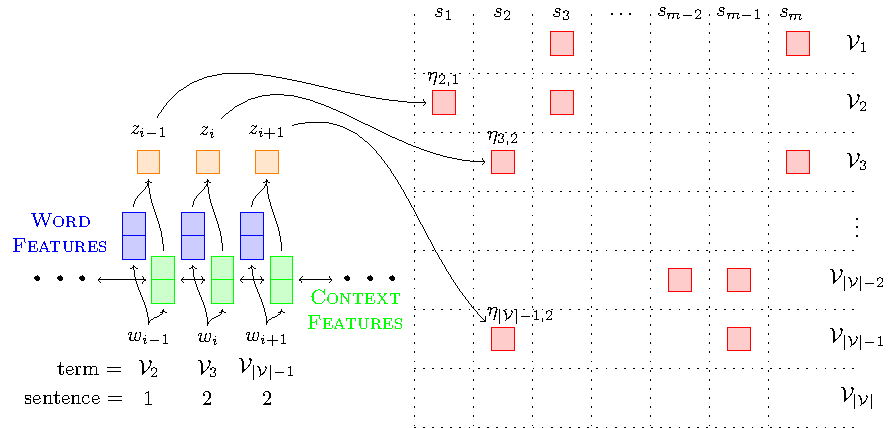
\includegraphics[scale=.7]{chapter4/figures/4_2_wimp_model.pdf}
 \end{center}
\caption{Left: Word and context features are extracted from the flat token
sequence representation to get word level importance scores 
$\wordImportance_i$. Right: word level scores are aggregated into a sparse
bag-of-words representation of the input sentences.}
\end{figure}

Our previous experiments revealed that lexical sematics were not the 
main driver of learning in sentence extractive news summarization. 
One could plausibly argue that it is a feature, not a bug, and that 
the structural
signals in news are intentional and not to be avoided. However, we think more 
attention could be paid to estimating importance scores at the word level.
We are motivated by potential application to abstractive generation: better
word level importance estimation could help to remove all but the most 
necessary content from the documents as a preprocessing stage before
abstractive summarization. We are also encouraged by parallel practices
in multi-lingual news summarization, where word importance weights 
are the main ingredient in sentence representations. 


\newcommand{\mlingsys}{\textsc{Classy}}

%\subsubsection{A brief discussion of \mlingsys.}

\mlingsys and its antecedents have been consistent top performers in various
summarization workshops \cite{tac,multiling}. In general the main approach 
is to represent each sentence as a sparse bag-of-words, where non-zero
entries correspond to word importance weights for the words found in the 
sentence. Typically, tf-idf weights are used for the importance scores.
The term by sentence matrix representing the document or documents to be
summarized is then factorized into two low rank matrices (typically with
non-negative entries) representing term factors and sentence factors.
The entries in the sentence factor matrix represent latent factors, 
and apriori the importance of each sentence is the sum of its latent factors.

Sentence selection can subsequently be performed using one of several methods.
In the naive case, one can select the sentence with the highest vector norm, 
substract the selected latent factors from the remaining sentence vectors
(zeroing out any terms that become negative), and repeating until the
summary length budget is reached. More sophisticated selection procedures
involving multi-dimensional knapsack packing or submodular optimization 
can be used, however these are not the focus of this work.

One draw back to this approach is that the sentence factors and word 
importance scores are unsupervised with respect to the final summarization
objective; their utility to the summarization task is a happy coincidence.
Additionally, the word importance scores are not assigned based on the 
context in which the word appears.

We propose to address these issues by learning word level importance 
scores in the process of single document sentence extractive summarization.
Additionally, we propose a method of adapting these scores from the 
single document case to multi-document summarization.

\subsubsection{Proposed Model}


In our proposed model for word importance, we estimate the importance of
each word in the context it occurs by first running the ELMO model
over all the words in the document to obtain contextual representations
of each word. The ELMO embeddings are then combined with pretrained Glove
embeddings, document frequency embeddings, topic signature embeddings,
sentence position embeddings, and part-of-speech tag embeddings and then
fed into a multi-layer perceptron to predict a scalar importance score.
When a word occurs multiple times in the input, it can be given a different 
importance score at each location because the ELMO embeddings will capture
contributions of the salient neighbor words. A term-sentence matrix is 
then formed from the input, using the estimated word importance scores 
as the term weights. A sentence extractive summary can be obtained 
using the naive sentence selection method described above or in Figure ?.
The total score for the summary can also be obtained.

We can train this summarizer using a gold extract sequence and a margin loss
\[  \max\left(0, 1 + f(\hat{y}) - f(y) \right) \] where $f(\hat{y})$ is
the score of our predicted extract summary.


Let $z_1, z_2, \dots, z_n$ be the bag of words representations of the 
sentences selected for the summary, in the order they were selected.
The score for the summary is computed as 
$\textsc{Score}(z) = \sum_{i=1}^n \sum_{j=1}^k \max(0, z_{i,j} - \sum_{l=1}^{i-1} z_{l,j})$ 


~\\
~\\

Let $\vocab$ be a fixed vocabulary of words. A document is a sequence $m$
words $\word = \{\word_1, \word_2, \ldots, \word_m\} \in \vocab^m$.
We define two mappings of words to dense vector representations.
The first $\fdef{\wordFeatures}{\vocab}{\Rn{d_1}}$ maps words to 
a concatenation of feature embeddings whose total dimension is of size $f$. 
The various components of the feature embeddings include the word's Glove 
embedding, an embedding for sentence position, and other features of the word.
The second mapping
$\fdef{\contextFeatures}{\vocab}{\Rn{d_2}}$ maps the word to it's contextual
embedding; here this corresponds to the output of \elmo at that word's
position in the document. 
The importance score $\wordImportance_i$ of a word $\word_i$ is the output of 
a feedforward layer 
\[ \wordImportance_i = \sigma\Big(W \left[\begin{array}{c} \wordFeatures(\word_i) \\ \contextFeatures(\word_i) \end{array} \right] + b \Big) \]
    where $W \in \Rn{d_1 + d_2}$ and $b \in \R$ are learned weight
and bias parameters, and $\sigma$ is the logistic sigmoid.

Next, we aggregate the flat token level scores into a bag-of-words (BOW) 
representation for each sentence in the document.
Let $I_i$ be the set of indices of the flat word sequence corresponding
to the words in $i$-th input sentence. Let $\bow_i$ be the BOW 
representation of the $i$-th sentence with entries 
\[ \bow_{i,j} = \begin{cases} 
    0 & \textrm{if $\word_k \ne \vocab_j $ for all $k \in I_i $} \\ 
\sum_{k \in I_i} \mathbbm{1}\{\word_k = \vocab_j \} \cdot \wordImportance_k  & \textrm{otherwise}     \end{cases} \]
        for all $j \in \{1, \ldots, |\vocab|\}$.



\begin{figure}
  \begin{algorithmic}[1]
    \Procedure{\textsc{BowExtracter}}{$\bow, \beta, \kappa$}
   
      \State $\bow_i^{(1)}  \gets \bow_i \quad \forall i \in [[n]]$
      \State $\hat{\eta} \gets 0$
      \State $t \gets 0$
      \While{ $\sum_{i=1}^t \kappa_{\predLabels_i} < \beta$ and $t < n$}
        \State $t \gets t + 1$
        \State $\predLabels_t \gets \operatorname{arg max}_{i \in [[n]]}
            \sum_{j=1}^{|\vocab|} \bow^{(t)}_{i,j}$
        \State $\bow_i^{(t+1)} \gets \max(0, \bow_i^{(t)} - \bow^{(t)}_{\predLabels_t} )\quad  \forall i \in [[n]]$
        \State $\hat{\eta} \gets \hat{\eta} + \sum_{j=1}^{|\vocab|} \bow_{\predLabels_t,j}^{(t)}$
         

      \EndWhile
        \State \Return $[\predLabels_1,\ldots,\predLabels_t], \hat{\eta}$ \Comment{Returns summary sentence indices and summary score.}
    \EndProcedure
  \end{algorithmic}
\caption{Simple sentence extraction algorithm given non-negative BOW inputs.}
\label{alg:wimp_ext_alg}
\end{figure}



        With the BOW representations in hand, we perform sentence selection
        using the algorithm presented in \autoref{alg:wimp_ext_alg} to 
        obtain a predicted extract indices $\predLabels$ and their associated
        score $\hat{\eta}$.

        We can optimize this model using a margin loss, where given a 
        gold extract sequence  $\labels$, we can compute the associated
        gold extract summary score $\eta$ and then minimize the following
        loss function \[\mathcal{L}_{ext}(\predLabels, \labels;\theta) = \max\big(0, 1 + \hat{\eta} - \eta\big)\]
        with respect to the parameters of the word importance predictor.
        If needed, we can also introduce a supervised learning signal to the 
        individual word importance scores by collecting labels $\zeta_i$ for
        each $\wordImportance_i$ such that $\zeta_i = 1$ if $\word_i$ occurs
        and any human reference abstract and $0$ otherwise. For the word level
        loss we would use the cross entropy 
        \[ \mathcal{L}_{word}(\wordImportance, \zeta; \theta) = -\sum_{i=1}^m \zeta_i \log \wordImportance_i + (1 - \zeta_i) \log (1 - \wordImportance_i). \] 




        \paragraph{Adaptation to MDS} We also propose a simple 
        self attention-based modification to
        the word importance aggregation step to help adapt this method
        to multi-document summarization (MDS). \citep{conroy} found
        that dimensionality reduction on the BOW representations improves
        summarizer performance in the MDS setting (but not on single document
        summarization). 


        We plan to experiment with the following importance 
        aggregation method. First, given the outputs of the contextual features
        $h_i$, we compute a self attention matrix $\Lambda \in \Rn{m\times m}$
        where \[\Lambda_{i,j} = \sigma(h_i \cdot h_j / \tau + b)  \]
        using sigmoidal attention \cite{strucattn} with a learned bias 
        parameter $b$ and a temperature parameter $\tau$.
        Next we compute an attention weighted word importance score $\bar{\wordImportance}_i$ for each word in the input using the following formula,
        \[ \bar{\wordImportance}_i = \sum_{j=1}^m \wordImportance_j \cdot \Lambda_{i,j}.\]

        Our motivation is that by accumulating scores based on context
        similarity, words and topics that appear in multiple documents 
        will accumulate the bulk of the word importance scores, giving 
        an added boost to sentences that contain them. Implicitly, errant
        words from one document that are not on topic to the cluster will
        effectively not contribute much to a sentences score, reducing the 
        effectve dimension of the BOW vectors and regularizing individual
        sentences to the document cluster's mean.

        
        Since we are training our models on single documents, we expect that
        running our pretrainined word scoring model on the individual 
        documents from an MDS document cluster will result in 
        minimal task-adaptation mismatch. Remaining bias and temperature
        parameters can easily be tuned on the small amount of MDS training 
        data available.

        We also plan to compare this method to using a non-negative matrix 
        factorization 
        method on the output of the learned BOW representation, 
        and to hard attention assignments using Brown clustering.







%\subsubsection{
%\cite{conroy} 


 

}{}



\bibliographystyle{plainnat}
\bibliography{cites}

\end{document}
